\documentclass{article} % For LaTeX2e
\usepackage[utf8x]{inputenc}  % adding the UTF-8 encoding
\usepackage[hebrew,english]{babel}     % Hebrew is primary, English is secondary
\usepackage{graphicx}
\graphicspath{ {images/} }
\usepackage{nips14submit_e,times}
\usepackage{hyperref}
\usepackage{cleveref}
\usepackage{subcaption}
\usepackage{url}
%\documentstyle[nips14submit_09,times,art10]{article} % For LaTeX 2.09

\title{Automatic Target Detection and Classification: \\
  Deep Learning on Low Power Platforms \\
  \begin{otherlanguage}{hebrew}
    זיהוי וסיווג אוטומטי של מטרות: \\
    למידה עמוקה על פלטפורמה נמוכת הספק
  \end{otherlanguage}
}

\author{
  Asst. Prof. Mark Silberstein \\
  mark@ee.technion.ac.il\\
}

\newcommand{\fix}{\marginpar{FIX}}
\newcommand{\new}{\marginpar{NEW}}

\nipsfinalcopy % Uncomment for camera-ready version

\newcommand{\cropsrow}[3]{\includegraphics[width=0.15\textwidth]{images/crops/#1.jpg} & #2 & \includegraphics[width=0.15\textwidth]{images/crops/mask_#1.jpg} & #3}

\begin{document}

\maketitle

\section{Summary}

Over the last decades the use of Unmanned System (US) has proved very beneficial
in saving life of military personal and cutting the costs of operational tasks.
However, these systems still require a `Man in the loop' for remote control,
scene recognition, and data acquisition, thereby increasing the cost of
operation and significantly limiting the scope of applications to those in which
such a remote control is possible.

On the other hand, recent years have seen revolutionary advancements in machine
learning algorithms. The new class of algorithms, called Deep Neural Networks
(DNN), has been shown to enable computers accomplish image classification and
recognition tasks previously considered tractable only by humans. The tremendous
potential of these algorithms in solving recognition tasks in Unmanned Systems
is apparent, as their use may bring real-time human-level vision capabilities
and pave the way toward fully Unmanned Autonomous Systems (UAS). Unfortunately,
the typically scarce computing capacity of unmanned systems, primarily due to
strict weight and size constraints, make the application of the existing
compute-greedy deep neural network-based algorithms extremely challenging.

This proposal aims to bring the power of deep neural networks to Unmanned
Systems via two main research thrusts:

\begin{itemize}
\item Optimization of the structure of deep neural networks for specific
	tasks encountered in (US), like target detection, object recognition,
	mapping, localization and more.
\item Optimization of the design and implementation of inference in deep neural
	networks with the focus on power efficiency. We will leverage a new  class of high
	performance low-power commodity platforms with embedded Graphics
	Processing Units (GPUs), like  NVIDIA Jetson TX1.
\end{itemize}

Deep neural networks-based systems achieve  state-of-the-art results in numerous
areas, yet, require considerable computing power. The need to satisfy the size and
power constraints of UAS requires finding the optimal balance between
mission requirements and algorithm performance. We will explore different
deep learning networks and compare them by their latency, throughput and
accuracy.

In this proposal we seek to take advantage of a novel hybrid CPU-GPU architecture of embedded GPUs
to leverage their computing capacity for low-power \emph{inference} in deep
neural networks. GPUs are now routinely used as high-performance
accelerators in supercomputing workloads, and in particular, for training deep
neural networks. Combined with the new generation of low power
embedded systems like NVIDIA Jetson TX1,  our work on power-optimized
inference holds the potential to empower complex classification and recognition
tasks on the Unmanned System.

Critically, throughout the intermediate stages of this project as well as upon
its completion, the progress will be evaluated on a real Unmanned Aerial Vehicle (UAV), in
cooperation with the Technion AUVSI project team which is a collaboration
between the Aerospace and Electrical Engineering departments.

\section{Background}

\subsection{Deep Learning}
\label{sec:deep_learning}

Classical machine learning, traditionally approaches classification problems by
first transforming the data from the problem space to some feature space. The
data in this feature space is hopefully invariant to transforms common in the
problem space, e.g. similarity and affine transforms, occlusion, lighting etc.
It is assumed that in this feature space, objects of the same class reside in
some manifold and the manifolds of different objects are separated by regions of
low density. A classifier, e.g. SVM, is trained on this feature space to
discriminate between objects of different classes.

This approach has been applied successfully to problems in many fields. But
finding the right feature space for the problem and the right classifier for the
feature space is a complicated task that requires expertise.

In the last years, Deep Neural Networks (DNN)~\cite{Bengio2009, LeCun2015} proved to
be the best machine learning technique for  many artificial intelligence
tasks~\cite{hadsell2009learning, eigen2014depth, ross2013learning}. One of the
main advantages of DNN is that the automatically learn the feature space. Thus
the feature space is custom tailored for the specific problem.

\subsection{General-purpose computing on graphics processing units}

General-purpose computing on graphics processing units is the use of a graphics
processing unit (GPU),to perform computation in applications traditionally
handled by the central processing unit (CPU). The advantage of GPUs over  CPUs
comes from the massive hardware parallelism, which enables high throughput and
unprecedented performance in a variety of parallel tasks, well beyond the
computer graphics domain. GPUs particular excel at linear algebra tasks like
matrix product, which lie in the heart of Deep Neural Network training and
inference. Therefore,  GPUs have been shown extremely effective for speeding up
DNN training, achieving  up to an order of magnitude  faster execution than the
CPU.

\subsection{AUVSI project}

The Association for Unmanned Vehicle Systems International (AUVSI) organizes the
Student Unmanned Aerial System (SUAS) competition
\url{http://www.auvsi-seafarer.org/}. The competition is aimed  at stimulating
and fostering interest in unmanned system technologies. The  students  are
required  to  develop  and  provide  the  analysis, design, fabrication and
demonstration of a system capable of completing specific autonomous aerial
missions.

One of the missions is the automatic detection and classification of targets.
Some targets are characterized by different geometric shapes and color. A specific
target, in the form of a QR code requires high spatial resolution. Another
target is a doll in the form and size of a human. This target simulates a search
and rescue operation.~\cref{fig:targets} shows some of the targets used in last
year's competition.
\begin{figure}[h]
	\centering
	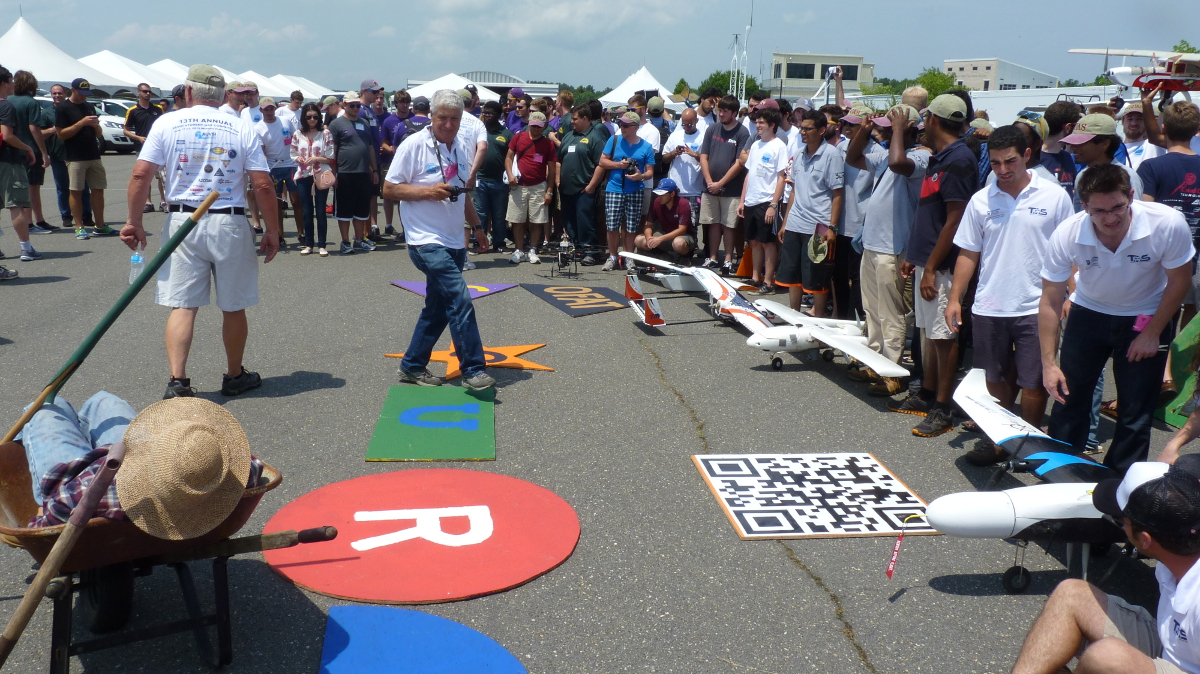
\includegraphics[width=0.8\textwidth]{auvsi_targets}
	\caption{Example of targets used in the 2015 AUVSI competition.}
	\label{fig:targets}
\end{figure}

This is the third year that the Technion participates in the AUVSI SUAS
competition. Last year the Technion team achieved 2\textsuperscript{nd} place
among more than 30 teams from universities all around the world.

\section{Proposed Research}

\subsection{Target Detection and Classification}
\label{sec:target_detect_and_class}

The task of target detection and classification is related to surveillance,
`search and rescue', `friend or foe' identification and many other security
related missions. The Regions with Convolutional Neural Networks
(R-CNN)~\cite{Girshick2014}, introduced in 2014 ,revolutionized the area of
object detection, classification, and segmentation. Fig.~\ref{fig:RCNN} shows the
diagram of a typical R-CNN system. It is made of two stages, the first is a
region proposal stage that extracts object candidates. This regions are
stretched into a predefined patch size and then fed into a CNN. The CNN
calculates confidence levels for a set of objects it was trained for.
\begin{figure}[h]
	\centering
	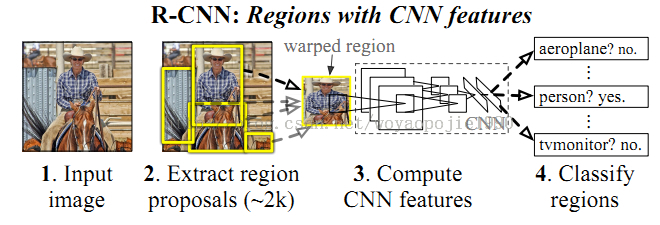
\includegraphics[width=0.8\textwidth]{RCNN}
	\caption{Diagram of a RCNN system}
	\label{fig:RCNN}
\end{figure}

DNNs hold the potential to perform well on this task, and we propose to extend
existing algorithms in multiple directions. For one, we will explore
methods for making the classification robust to different light and weather
conditions. We will also train the network to detect and classify targets among
cluttered and diverse backgrounds. The key requirement for achieving this level
of robustness is large training dataset. In collaboration with AUVSI team we
will collect aerial imagery at different locations and weather conditions. Also, as detailed
in~\cref{sec:low_power_computing}, most of the computing time is spent in the detection
stage. Our goal is to achieve Real-Time detection at video frame rate. Therefore we will
explore methods for performing detection using a DNN~cite{Szegedy2013}.
For example we will test merging the detection and classification stages into a
single network~\cite{long2014fully}.

\subsubsection{Preliminary results}
We implemented a system based on the R-CNN architecture to detect and classify
the targets. In our preliminary system the detection is done using the Maximally
Stable Extremal Regions (MSER) algorithm~\cite{Forssen2007}. The classification
is divided in two hierarchical Convolutional Neural Networks (CNNs). The CNNs are shown
in~\cref{fig:shape_diagram} and~\cref{fig:letter_diagram}.

\begin{figure}[h]
	\centering
	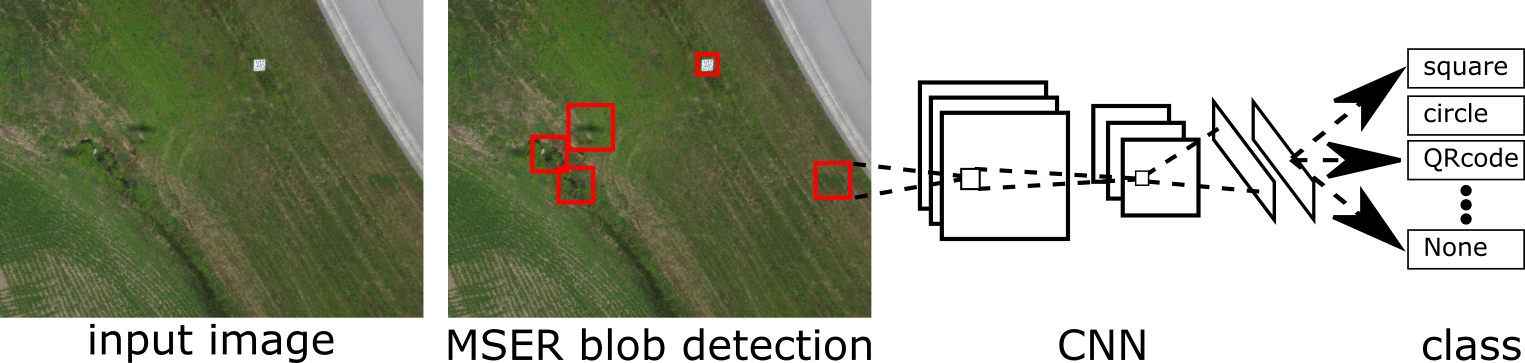
\includegraphics[width=0.8\textwidth]{diagram}
	\caption{Diagram of the shape classification subsystem}
	\label{fig:shape_diagram}
\end{figure}
\begin{figure}[h]
	\centering
	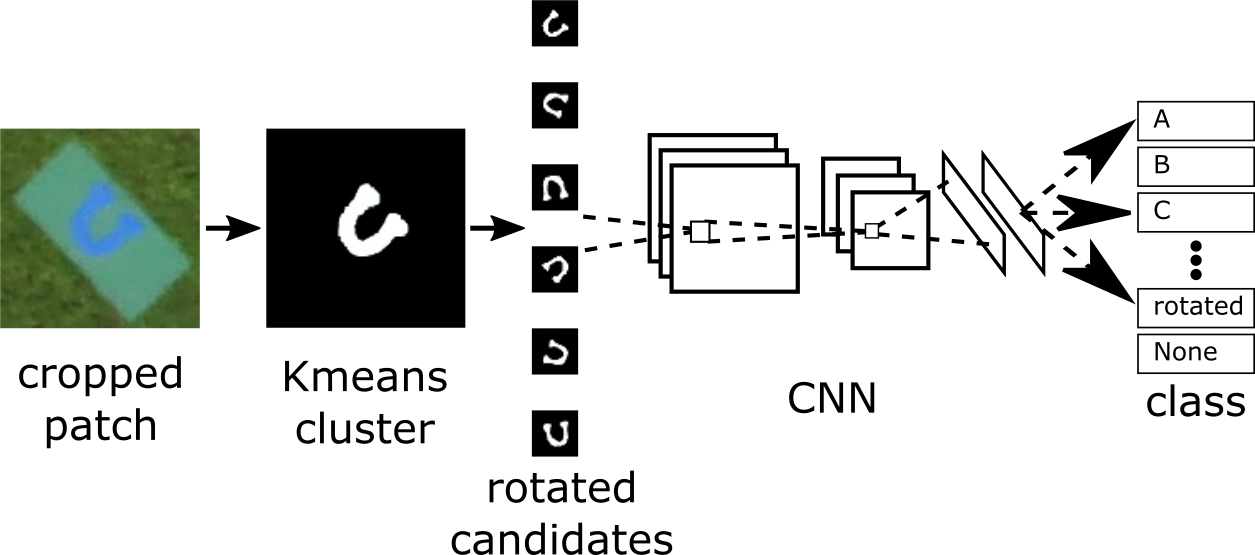
\includegraphics[width=0.5\textwidth]{letter_diagram}
	\caption{Diagram of the character classification subsystem}
	\label{fig:letter_diagram}
\end{figure}

The first CNN detects and classifies target shapes in the full (downscaled)
image. The input to this CNN is a down-sampled version of the original
image. The outputs are square regions classified as one of the possible target
shapes (circle, half circle, cross, rectangle, etc.). These regions are cropped
from the full resolution image and fed into the next CNN that classifies
the characters inside the shape. These CNNs thus work as a cascade of
classifiers. This hierarchical structure enables good classification
performance using smaller DNNs. \Cref{fig:true_positive2} shows
results of automatic detection and classification using this system.

\begin{figure}[h]
	\centering
	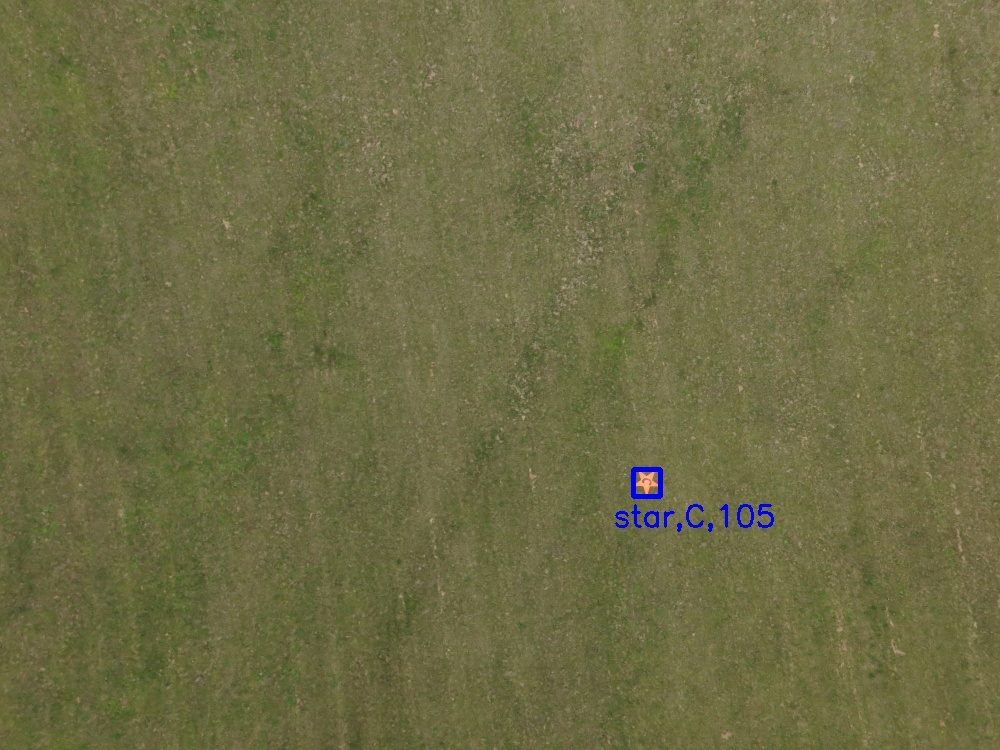
\includegraphics[width=0.8\textwidth]{true_positive_correct_letter2}
	\caption{Target classified correctly as: shape=star, char=C and angle=$105^\circ$.}
	\label{fig:true_positive2}
\end{figure}


\subsection{Low Power Computing}
\label{sec:low_power_computing}

The Jetson TX1,~\cref{fig:jetson}, and its predecessor, the Jetson
TK1~\cite{jetsontk}, offer both a general purpose CPU and a powerful GPU in a
low power ($<10[\textrm{W}]$), small form factor platform
($10\textrm{x}10[\textrm{cm}]$). The GPU enables fast inference in Deep
Learning Networks. Using the Jetson TX1 and the Caffe~\cite{jia2014caffe} DNN
development network, we propose to  develop a low power, real-time target detection and classification
system.

\begin{figure}[h]
	\centering
	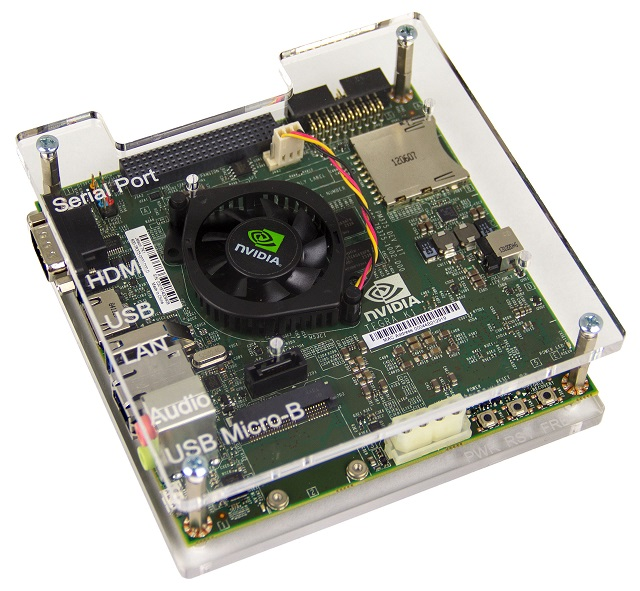
\includegraphics[width=0.8\textwidth]{jetson}
	\caption{The Jetson TK1 by NVIDIA}
	\label{fig:jetson}
\end{figure}

\subsubsection{Preliminary results}
Initial results of running the target detection and classification algorithm on
the older Jetson platform are shown in~\cref{tb:jetson1}. It can be seen that even at this
stage the system can handle images at up to 4 frames per second, yet this frame
rate is too slow.
\begin{table}
	\centering
	\begin{tabular}{ | l | l | }
		\hline
		Stage                                & Time [ms] \\ \hline
		Target Detection (CPU)               & 183       \\ \hline
		Low Resolution Classification (GPU)  & 7         \\ \hline
		High Resolution Classification (GPU) & 15        \\ \hline
		Total                                & 215       \\ \hline
	\end{tabular}
	\caption{Timing results on the Jetson TK1}
	\label{tb:jetson1}
\end{table}

To explore network optimization strategies we run a computationally demanding
DNN called `AlexNet' on the Jetson TK1. Results of profiling the
`AlexNet'~\cref{fig:alex_time} show that more than $35\%$ of the classification
time is spent in one of the network layers (`FC6'). \Cref{tb:alexnet} details
the improvement in classification time VS Accuracy hit for different
modifications to the network architecture.
\begin{figure}[h]
	\centering
	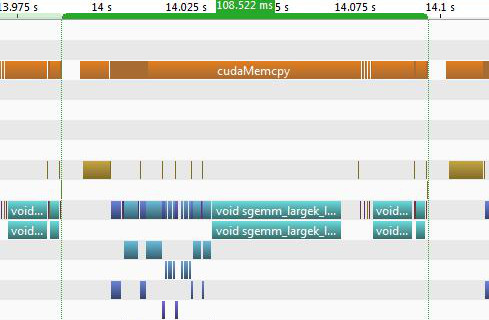
\includegraphics[width=0.8\textwidth]{alexnet_time_line_small}
	\caption{Profiling of the AlexNet DL network}
	\label{fig:alex_time}
\end{figure}
Our preliminary results show that it is possible to decrease the size of the
network  while maintaining an acceptable accuracy.
\begin{table}
	\centering
	\begin{tabular}{ | l | l | l | l | }
		\hline
		                    & Classification Time [ms] & Top-1 Accuracy & Improvement \\ \hline
		Original AlexNet    & 106                      & 57\%           & 1           \\ \hline
		FC6=2048            & 73                       & 54\%           & X1.45       \\ \hline
		No FC6              & 95                       & 55\%           & X1.13       \\ \hline
		64x64 inuput images & 57                       & 50\%           & X2          \\ \hline
	\end{tabular}
	\caption{Timing results on the Jetson TK1}
	\label{tb:alexnet}
\end{table}

Further improvements can be achieved by optimizing the code of the DNN framework
in use. In our tests we were able to reduce the classification time by $15\%$ by
optimizing the code of the CAFE framework we use~\cite{jia2014caffe}.

As can be seen in table~\cref{tb:jetson1}, the target detection stage is by far
the most time consuming. We will explore methods for optimizing the performance
of this pipeline. These methods include porting of the CPU tasks to the GPU by
merging the detection and classification stages. Another direction is developing
custom CUDA kernels~\cite{nvidiacuda} to replace the time consuming parts.

\subsection{Evaluation and Integration with Real-World Systems}

The developed algorithms will be tested on the `Technion
drone'~\cref{fig:drone}. This project is developed as part of the Association
for Unmanned Vehicle Systems International (AUVSI) Student Unmanned Air Systems
(SUAS) Competition~\cite{AUVSI_competition}.
\begin{figure}[h]
	\centering
	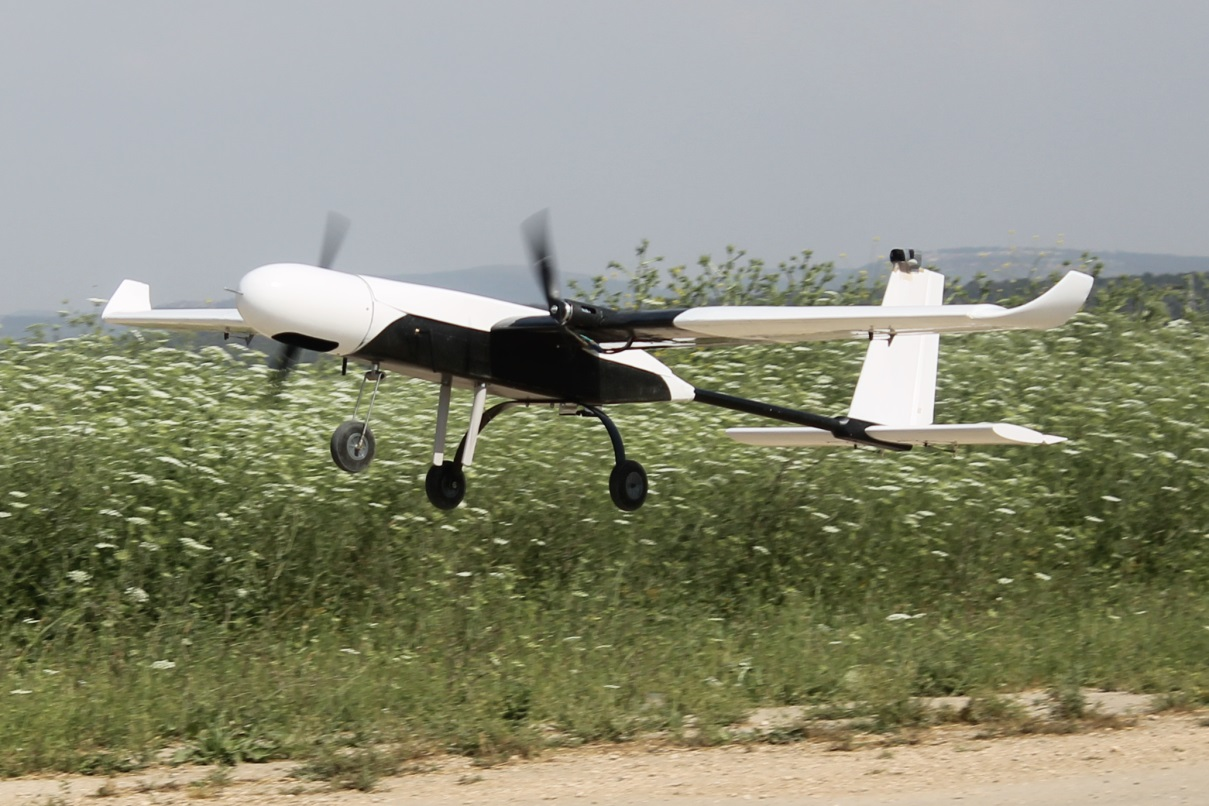
\includegraphics[width=0.8\textwidth]{drone}
	\caption{The Technion drone project.}
	\label{fig:drone}
\end{figure}
The `Technion Drone' is an annual multidisciplinary project in which students
from both faculties - Aerospace Engineering and Electrical Engineering team
together to develop an Unmanned Aerial system, a system capable of conducting
air operations which include autonomous flight and navigation, and use of
onboard payload sensors (to be developed by the students) to execute specified
tasks. During the project the students experience team-work under intensive
supervision and perform the following tasks: Design and Analysis, Fabrication,
Ground and Flight testing, flight Demonstration of the UAS, and reporting all
the above in a detailed and concise report.
\begin{figure}[h]
	\centering
	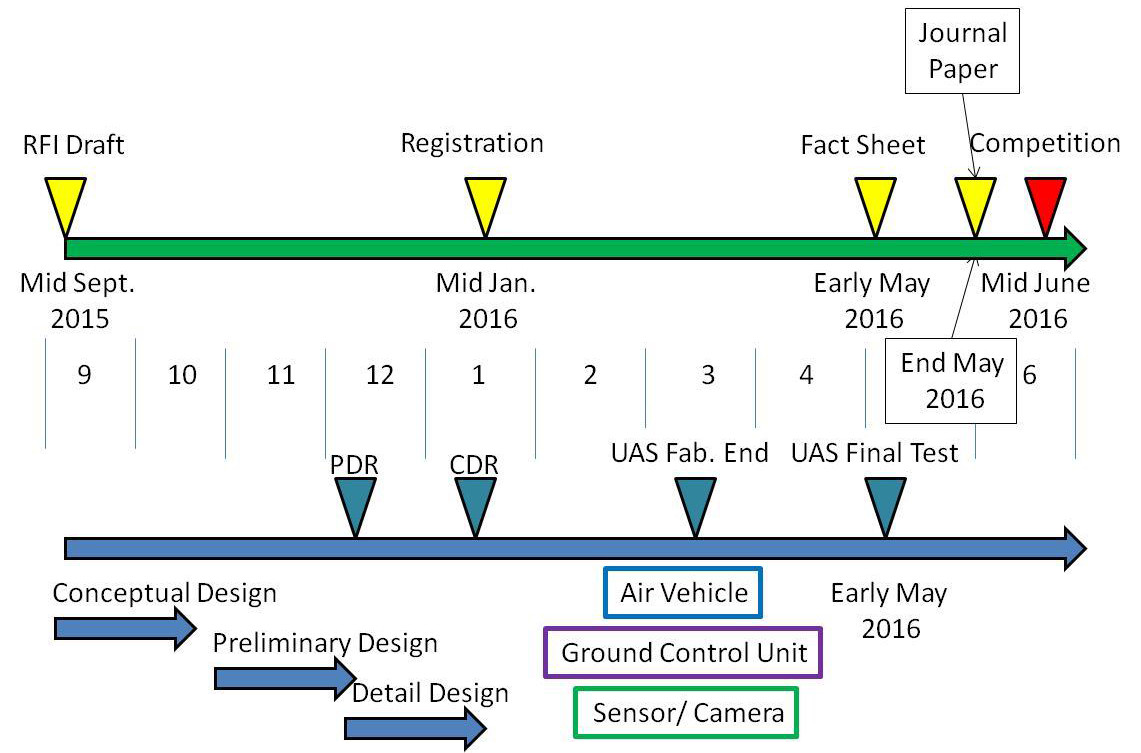
\includegraphics[width=0.8\textwidth]{project_timeline}
	\caption{Timeline of the 2016 Technion Drone project.}
	\label{fig:drone}
\end{figure}
The highlight of this challenging,
multidisciplinary project is the participation in the leading and most
prestigious students competition (which includes leading Universities from around
the World), which takes place in the USA. Last year (2015) the Technion team
achieved 2\textsuperscript{nd} place.

The `Technion Drone` was presented by the students in several conferences
including the UVID-International conference on Unmanned Vehicles which is
organized by `ISRAEL DEFENSE MAGAZINE'. The project won a special Academic Prize
for outstanding academic achievements.

This year, a Jetson TX1 mini computer will be deployed on-board the drone as part of
its payload. It will process images captured by the payload camera in real time.
Among its tasks will be  automatic detection and classification of targets
and the detection of humans. As the project evolves, more tasks will be
transfered from the ground station to the drone , e.g. Localization and Mapping~\cite{Nardi2014},
Obstacle Avoidance~\cite{Michels2005} allowing
autonomous capabilities to the drone.

\section{Budget Plan}

\begin{center}
	\begin{tabular}{ | l | l | l | }
		\hline
		      & Item                                                       & Budget (NIS) \\ \hline
		1     & MSc Student                                                & 50,000       \\ \hline
		2     & Optical payload with global shutter machine vision cameras & 30,000       \\ \hline
		3     & 1 computer and accessories                                 & 10,000       \\ \hline
		4     & 4 GPU Nvidia Jetson TX1                                    & 12,000       \\ \hline
		5     & Operating expenses (Flight tests)                          & 15,000       \\ \hline
		6     & Supplies and publication                                   & 8,000        \\ \hline
		7     & Transportation and communication                           & 5,000        \\ \hline
		8     & Students travel                                            & 20,000       \\ \hline
		9     & Laboratory staff (engineers \& technicians)                & 20,000       \\ \hline
		Total &                                                            & 170,000      \\ \hline
	\end{tabular}
\end{center}

\section{Mark Siberstein - Short Biography}
Mark Silberstein is an assistant professor at the Technion Electrical
Engineering Department, where he heads the Accelerated Computing Systems
Laboratory.  Mark is an internationally recognized expert in GPU computing, accelerated computing systems,
Operating Systems and high performance computing.  Mark's work has been published in more than
20 prestigious international conferences and journals, and has been cited in
over 600 academic papers. Recently Mark has taught a graduate course on the
design and implementation of  neural networks, and currently supervises three
undergraduate projects and graduate research  on power efficient inference and distributed
training of DNNs.

\bibliography{project}
\bibliographystyle{unsrt}
\end{document}




%%% Local Variables:
%%% mode: latex
%%% TeX-master: t
%%% End:
